\documentclass{article}
% Chinese
% \documentclass[UTF8, nofonts, mathptmx, 12pt, onecolumn]{article}
% \usepackage{xeCJK}
% \setCJKmainfont{SimSun}
\usepackage{amsmath}
\usepackage{amsfonts}
\usepackage{amssymb}
\usepackage{wasysym}
% \usepackage{ctex}
\usepackage{graphicx}
\usepackage{float}
\usepackage{geometry}
\geometry{a4paper,scale=0.8}
\usepackage{caption}
\usepackage{subcaption}
% \newcommand{\oiint}{\mathop{{\int\!\!\!\!\!\int}\mkern-21mu \bigcirc} {}}
\newcommand*{\dif}{\mathop{}\!\mathrm{d}}
\newcommand*{\md}{\mathop{}\!\mathrm{d}}
\newcommand*{\me}{\mathrm{e}}

\usepackage{parskip}
\setlength{\parindent}{0cm}

\usepackage{bm}
\let\Oldmathbf\mathbf
\renewcommand{\mathbf}[1]{\boldsymbol{\Oldmathbf{#1}}}
\let\eqnarray\align

\author{Xiping Hu}
\usepackage{authblk}
\author{Xiping Hu}
\affil{http://thehxp.tech/}
\title{Homework for Analogue Electronics}

\begin{document}
\maketitle

\begin{figure}[H]
  \centering
  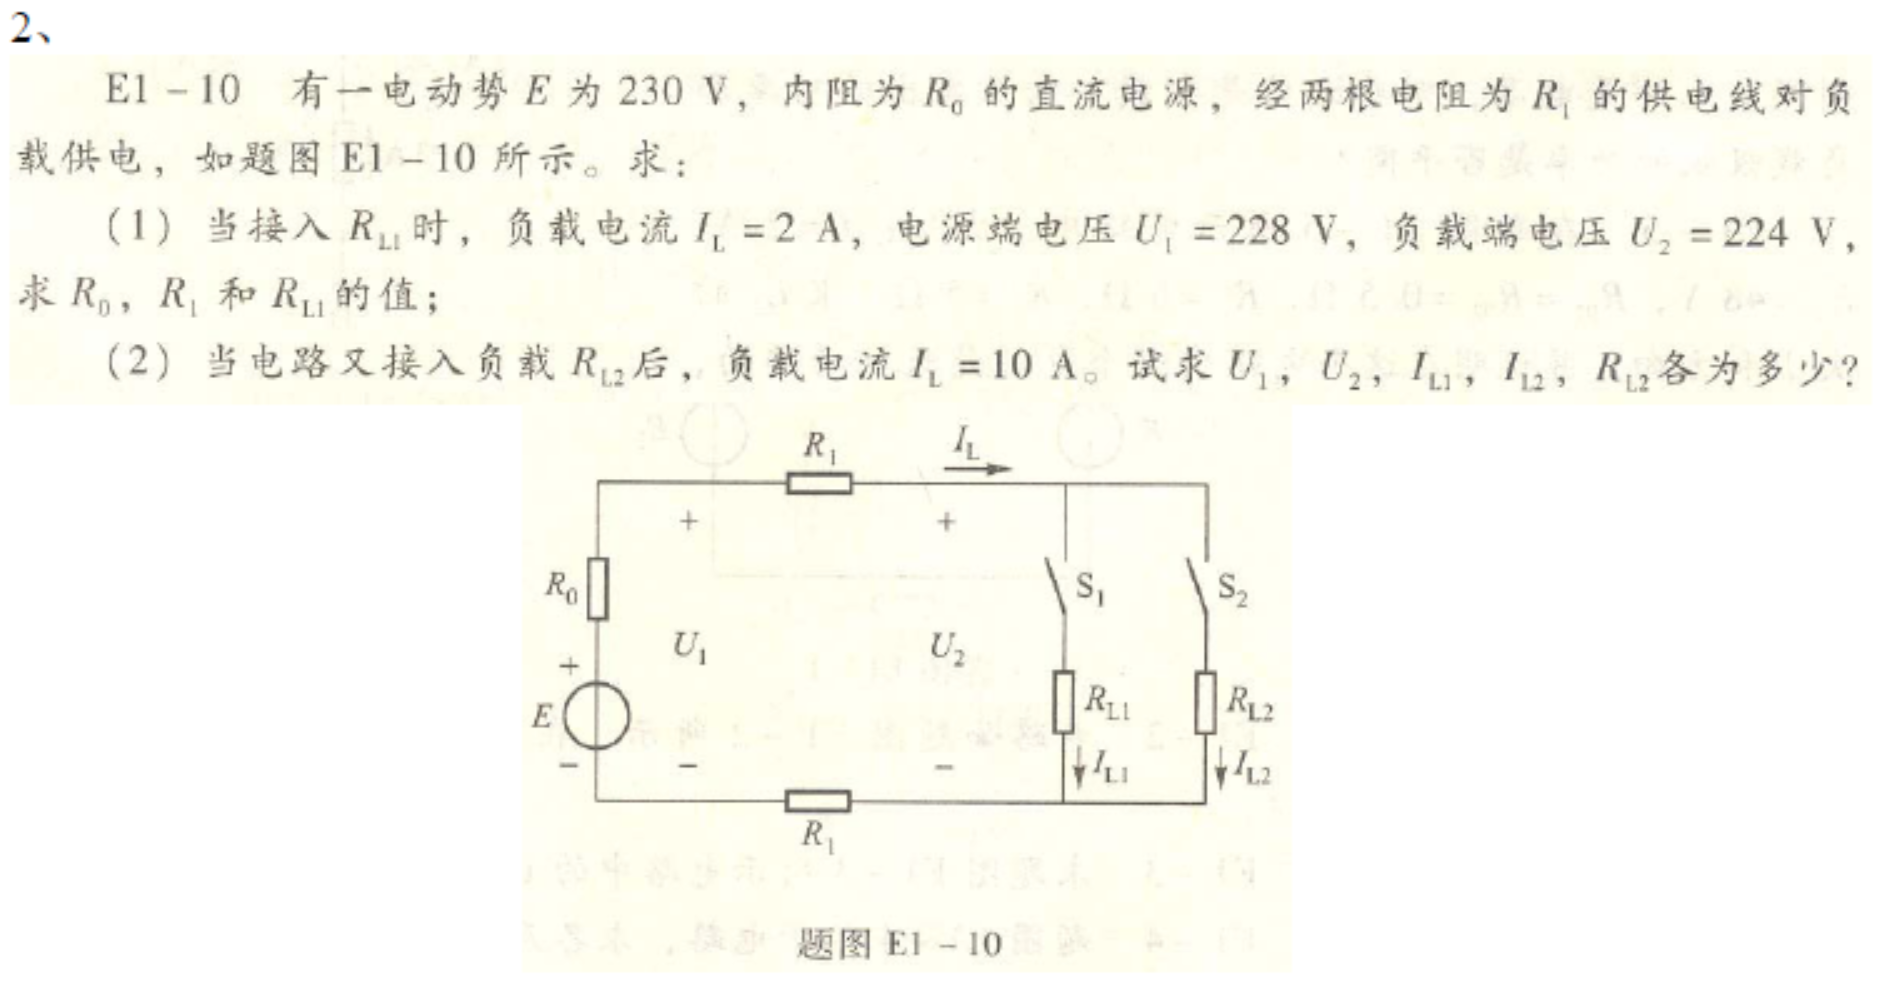
\includegraphics[width=\linewidth]{figures/2}
  \label{fig:}
\end{figure}

\paragraph{Solution for question 1}

When $S_1$ is closed
\begin{equation*}
  \begin{aligned}
    U_1 - I_L ( 2 R_1 ) - U_2 = 0 \\
    E + I_L R_0 = U_1 \\
    U_2 = I_L R_{L1}
  \end{aligned}
\end{equation*}

\begin{equation*}
  \begin{aligned}
    R_1 &= 1 \  \Omega \\
    R_0 &= 1 \  \Omega \\
    R_{L1} &= 112 \ \Omega
  \end{aligned}
\end{equation*}

\paragraph{Solution for question 2}

The parallel resistance of $R_{L1}$ and $R_{L2}$ is
\begin{equation*}
  \begin{aligned}
    R = \dfrac{R_{L1} R_{L2}}{R_{L1} + R_{L2}} 
  \end{aligned}
\end{equation*}

From the Kirchhoffs Voltage Law
\begin{equation*}
  \begin{aligned}
    E - I_L R_0 = U_1 \\
    I_L R = U_2 \\
    E - I_L \left( R_0 + 2 R_1 + R \right) = 0
  \end{aligned}
\end{equation*}

From which we can get

\begin{equation*}
  \begin{aligned}
    R = 20 \  \mathrm{\Omega} \\
    U_1 = 220 \  \mathrm{V} \\
    U_2 = 200 \  \mathrm{V}
  \end{aligned}
\end{equation*}

\begin{equation*}
  \begin{aligned}
    I_{L1} = \dfrac{U_2}{R_{L1}} = 1.79 \  \mathrm{A} \\
    I_{L2} = I_L - I_{L1} = 8.21 \  \mathrm{A} \\
    R_{L2} = \dfrac{U_2}{I_{L2}} = 24.36 \  \mathrm{\Omega} 
  \end{aligned}
\end{equation*}



\end{document}